% Chapter Template

\chapter{Implementation} % Main chapter title

\label{Chapter4} % Change X to a consecutive number; for referencing this chapter elsewhere, use \ref{ChapterX}

In this chapter, the overall structure of the project, how the files are arranged and the functionalities of each components, will be described in details.

%----------------------------------------------------------------------------------------
%	SECTION 1
%----------------------------------------------------------------------------------------

\section{Files And Folders}

The folder names and file names are mostly self-explanatory or conventional in this project. They'll be described briefly in this section.

\begin{figure}[th]
\centering
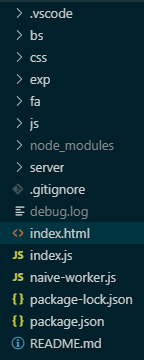
\includegraphics{Figures/Chapter4/filestructure.png}
\decoRule
\caption[File Structure]{A glimpse of files and folders.}
\label{fig:filestructure}
\end{figure}

\subsection{Folders}

\paragraph{Folder \texttt{./.vscode}}

\paragraph{Folder \texttt{./js}}

\paragraph{Folder \texttt{./css}}

\paragraph{Folder \texttt{./fa}}

\paragraph{Folder \texttt{./bs}}

\paragraph{Folder \texttt{./node\_modules}}

\paragraph{Folder \texttt{./exp}}

\subsection{Top Level Files}

\paragraph{File \texttt{index.html}}

\paragraph{File \texttt{index.js}}

\paragraph{File \texttt{naive-worker.js}}

\paragraph{File \texttt{package.json}}

\paragraph{File \texttt{package-lock.json}}

\paragraph{File \texttt{README.md}}

\paragraph{File \texttt{.gitignore}}


%----------------------------------------------------------------------------------------
%	SECTION 1
%----------------------------------------------------------------------------------------

\section{Front End}

Since this project is a pure web project, the front end occupies a large portion of the codes.

%-----------------------------------
%	SUBSECTION 1
%-----------------------------------
\subsection{HTML Entry \texttt{index.html}}

The entry of the project is where this program gets started, in similar concept of the \texttt{main()} function in \texttt{C} or the \texttt{public static void main(String[] args)} function in \texttt{Java}. The entry point is a \gls{html} file and as expected named \texttt{index.html}. It introduces the front end structure of the project in raw.

First part of the \gls{html} file is the \texttt{<head>} part. In this part, the character set of this web page is defined as \emph{UTF-8}, the size of the entire \gls{html} document as fullscreen size, scaling not allowed and not shrinking to display its content.

\begin{verbatim}
<meta charset="utf-8">
<meta name="viewport" content="width=device-width,
    initial-scale=1, shrink-to-fit=no">
\end{verbatim}

And then all the needed \gls{css} files are included to end the \texttt{<head>} part. Besides the \gls{css} files which will be described in \ref{chap4:frontend-css}, the necessary \gls{css} files from third-party open source vendors are also included, including \emph{Bootstrap}'s \gls{css} part, \emph{FontAwesome} and \emph{MiniBar} \gls{css} assets.

The \texttt{<body>} part is the essential part of the \gls{html} entry, which describes the structure of what users can ``actually see''. It begins first with three \texttt{<div>} tags for the most important three parts of this project, the container for main background canvases, the container for mini-maps, and the container for the control panel floating on the top right corner of the \gls{ui} screen. The positioning, sizes and container behaviours of these \texttt{<div>}s are defined in the \gls{css} files which are already included. Before users set any effects up, these properties mostly come from the file \texttt{./css/common.css}.

\begin{figure}[th]
\centering
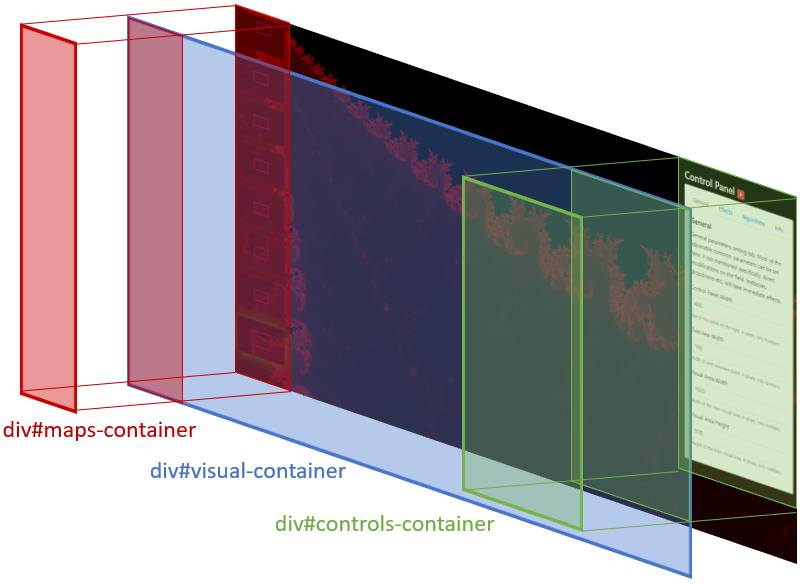
\includegraphics[width=\textwidth,keepaspectratio]{Figures/Chapter4/rootdom.png}
\decoRule
\caption[DOM Body Structure]{\gls{dom} structure in \texttt{<body>} tag.}
\label{fig:rootdom}
\end{figure}

After the visual \texttt{<div>} part, several \texttt{<script>} tags come after it to include what's necessary for the essential coding part. Here firstly are the dependencies of the project, including \emph{jQuery}, \emph{Bootstrap}'s \gls{js} part, and \emph{MiniBar}'s \gls{js} part. And then at the very end the main \gls{js} file \texttt{index.js} is included and all the core programs of this project goes in there.

Worth noting that conventionally all \gls{js} files should be included at the very end of the page as what we are doing now, unless the \gls{js} file is needed before the render phase of the web page. This way if the \gls{js} file is a little bit bigger than usual, the loading of the \gls{js} files won't affect the rendering process of the \gls{dom} documents.

%-----------------------------------
%	SUBSECTION 2
%-----------------------------------

\subsection{Main JavaScript \texttt{index.js}}

The main \gls{js} file \texttt{index.js} is where we put our core code, where we 

\subsection{CSSs For Overview Effects}
\label{chap4:frontend-css}

Folder \texttt{./css} includes five \gls{css} files, each setting up some visual effects of the project.

File \texttt{./css/common.css} first sets up all general apperance of the elements on the web page when no parameters or effects are set. File \texttt{./css/dock.css} sets up the apperance when \emph{Scrollbar + Dock} is activated, only the iOS Dock part and file \texttt{./css/minibar.css} sets up the scroll bar part. File \texttt{./css/stacked.css} sets up the effects of stacked cards. File \texttt{./css/tabs.css} sets up the effects of the tab selection on the top.

%----------------------------------------------------------------------------------------
%	SECTION 2
%----------------------------------------------------------------------------------------

\section{Back End Calculation}

The back end calculation is done in the \gls{js} file \texttt{naive-worker.js}. This file is being used for initializing the \emph{WebWorker}s inside \texttt{index.js} dynamically. Whenever a calculation or extraction for a specific region of a dataset is needed, the main \gls{js} file \texttt{index.js} is going to send a message to \texttt{naive-worker.js} with desired parameters and this back end will respond with corresponding image data.

\begin{figure}[th]
\centering
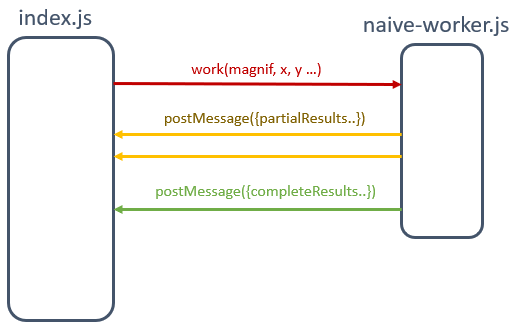
\includegraphics[width=\textwidth,keepaspectratio]{Figures/Chapter4/messageexchange.png}
\decoRule
\caption[Message Exchange]{Message exchange between \texttt{index.js} and \texttt{naive-worker.js}.}
\label{fig:messageexchange}
\end{figure}

\subsection{Global Scope}

In the global scope of this file, the following things were done.

\paragraph{Includes} The \texttt{decimal.js} dependency is included for high-precision floating points calculation. Default parameters for the dependency is set.

\paragraph{Constants} Constants of default screen width and default screen height are defined in case the front end doesn't give these parameters.

\paragraph{Canvas} An \texttt{OffscreenCanvas} instance is created and instantiated with the dimensions of by default the values of the defined constants. The \texttt{OffscreenCanvas} will be used as the canvas to generate the desired image on, and since it's not being shown on the screen, will occupy less system resources and boost the calculation speed. Corresponding variables is declared after the instantiation, respectively \texttt{canvas} for the \texttt{OffscreenCanvas} itself and \texttt{ctx} as the 2d context of the canvas.

\subsection{Message Reception}

\subsection{Iteration Limit}

\subsection{Iteration Count for One Point}

\subsection{Image Generation}

\subsection{High Precision Version}

\section{Utility Assets}

Other open source third-party utilities lie in different folders with corresponding names.

\subsection{Folder \texttt{./js}}

In \texttt{./js} folder, all \gls{js} third-party files are here, including:

\begin{itemize}
    \item File \texttt{decimal.min.js} is for high-precision floating points calculation for \glsdesc{js}.
    \item File \texttt{jquery-3.4.1.min.js} is for \gls{dom} traversal and manipulation, event handling and animation.
    \item File \texttt{bootstrap.bundle.min.js} is for some basic styling of the control panel sitting on top right corner of the screen.
\end{itemize}

\subsection{Folder \texttt{./fa}}

\subsection{Folder \texttt{./bs}}

\subsection{Folder \texttt{./css}}